\section{Industrialisierung und Aufbruch in die Moderne}

\subsection{Einführung: Industrialisierung als gesellschaftlicher Transformationsprozess}

Die Vorlesung betrachtet die Industrialisierung nicht nur als technische Entwicklung,
sondern als umfassenden gesellschaftlichen Wandel.

Industrialisierung bezeichnet jene Phase der wirtschaftlichen Entwicklung,
in der industrielle Produktion zur wichtigsten Triebkraft von Wachstum,
Innovation und gesellschaftlicher Veränderung wurde.

Dabei entstanden neue Technologien, Produktionsformen und Wirtschaftsstrukturen,
während traditionelle Formen der Herstellung und Arbeit an Bedeutung verloren. Gleichzeitig veränderten sich Lebensweisen, soziale Beziehungen und politische Verhältnisse grundlegend.

Zentrale Leitfragen:

\begin{itemize}
    \item Was versteht man unter Industrialisierung?
    \item Welche technischen und wirtschaftlichen Entwicklungen ermöglichten sie?
    \item Wie veränderte sich die Arbeitswelt?
    \item Welche gesellschaftlichen Folgen hatte die Industrialisierung?
\end{itemize}

Die Geschichte der Industrialisierung ist daher nicht nur Wirtschafts- und Technikgeschichte,
sondern auch Sozial-, Kultur- und Politikgeschichte.

\subsection{Das historiographische Problem der Industrialisierung}

Die Vorlesung betont, dass Industrialisierung kein einheitlicher Prozess war.

Vielmehr handelt es sich um eine komplexe Entwicklung,
die unterschiedliche Bereiche des gesellschaftlichen Lebens erfasste:

\begin{itemize}
    \item Produktionssysteme
    \item Technologien
    \item Ausbildung und Wissen
    \item Landschaften und Städte
    \item Arbeits- und Lebensweisen
\end{itemize}

Hinzu kommen erhebliche regionale Unterschiede.

Während manche Regionen bereits im 18. Jahrhundert industrialisiert wurden,
erlebten andere diesen Wandel erst deutlich später.

Auch die Perspektive der betrachteten Akteure beeinflusst die historische Darstellung:

\begin{itemize}
    \item Unternehmer
    \item Arbeiterinnen und Arbeiter
    \item Techniker
    \item Fabrikbesitzer
    \item Frauen und Kinder
    \item staatliche Kontrolleure
\end{itemize}

Die Industrialisierung lässt sich deshalb nicht auf eine einzige Ursache zurückführen.
Vielmehr wirkten wirtschaftliche, technische, politische und soziale Faktoren zusammen und beeinflussten sich gegenseitig.

\subsection{Protoindustrie im ostschweizerischen Textilgewerbe}

Vor der eigentlichen Industrialisierung existierten bereits arbeitsteilige Produktionsformen.

Besonders wichtig war in der Ostschweiz zwischen dem 16. und 18. Jahrhundert
das Leinwand- und Baumwollgewerbe.

Kennzeichnend waren:

\begin{itemize}
    \item Verarbeitung von Leinwand und Baumwolle
    \item Einbindung in weltweite Handelsnetzwerke
    \item starke Bedeutung des Zunftwesens
    \item arbeitsteilige Organisation der Produktion
\end{itemize}

Die Herstellung von Textilien erfolgte in zahlreichen einzelnen Arbeitsschritten,
die auf verschiedene Personen und Orte verteilt waren.

Dadurch entstand bereits vor der Industrialisierung eine komplexe Produktionsstruktur,
die als Protoindustrie bezeichnet wird.

\begin{center}
    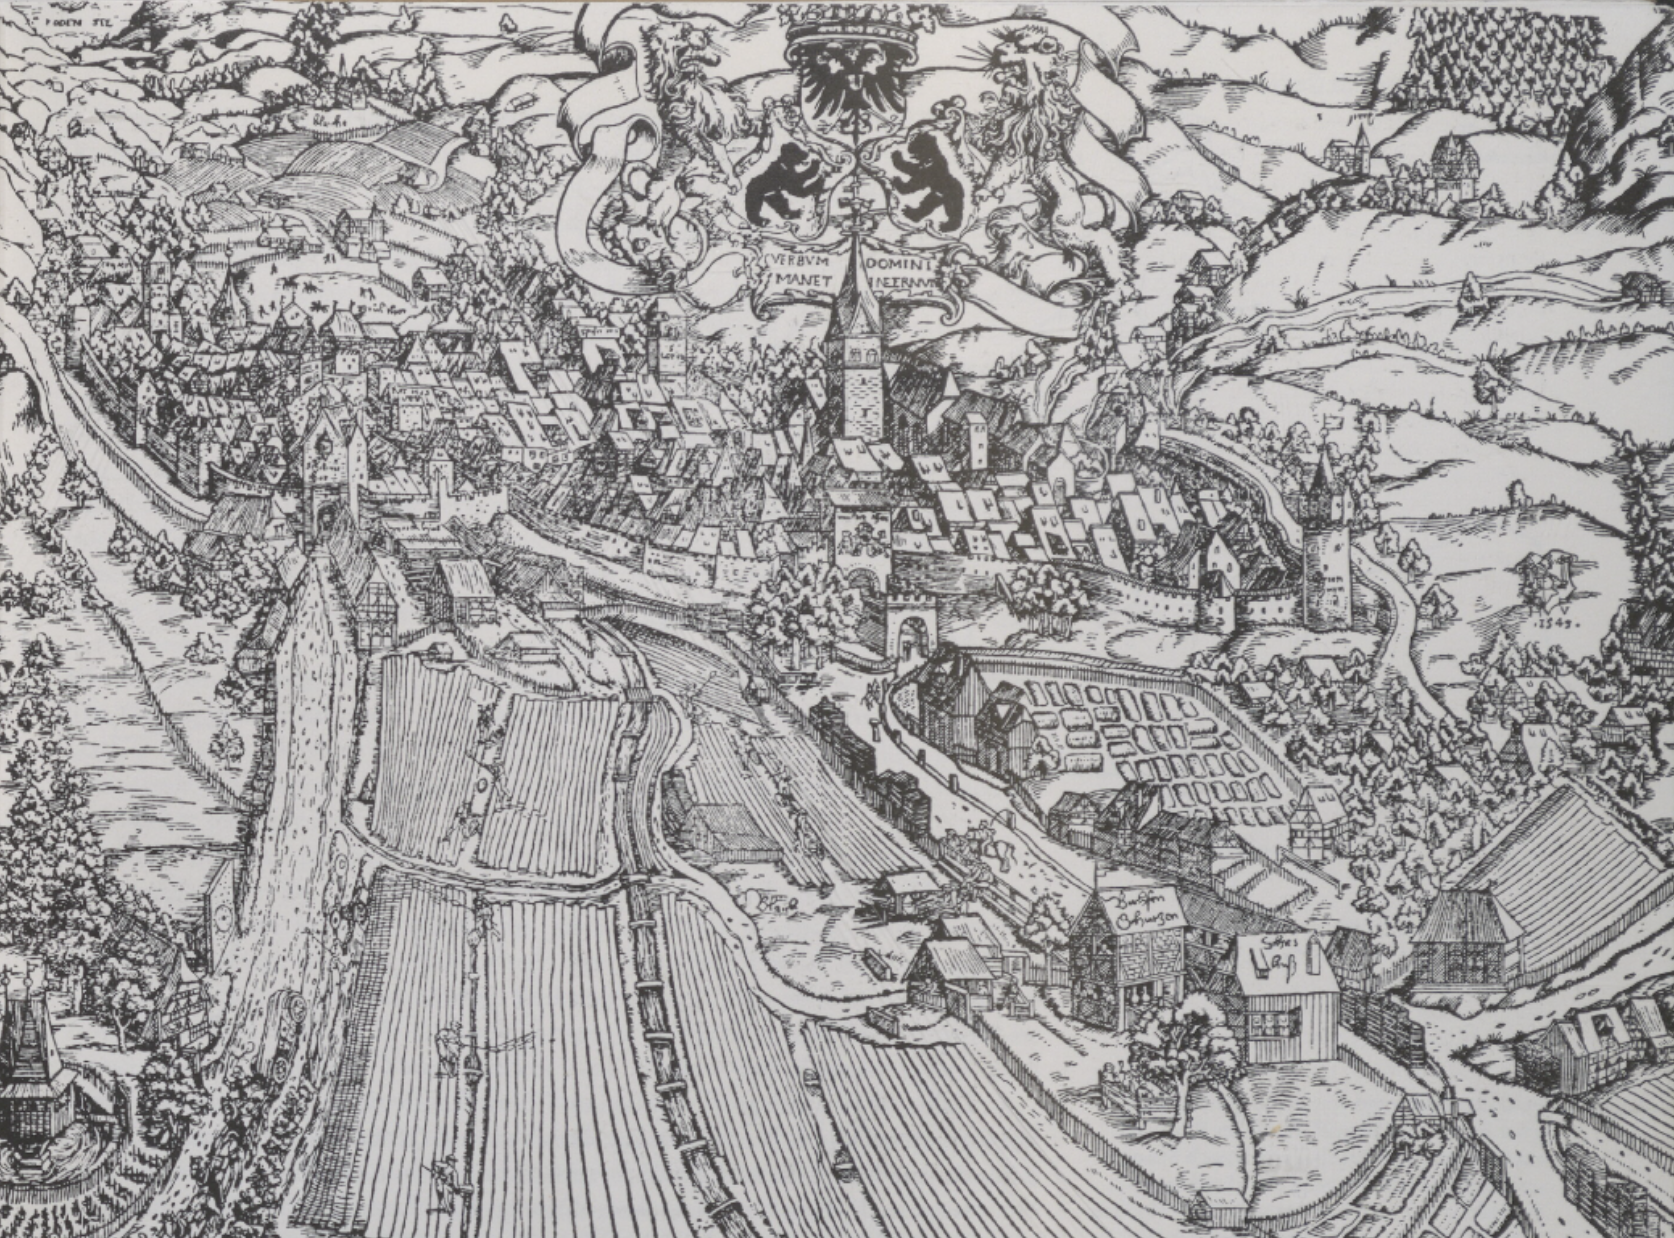
\includegraphics[width=0.8\linewidth]{images/st_gallen_1545.png}
\end{center}

\subsection{Produktion im Verlagssystem}

Die Textilproduktion beruhte überwiegend auf Heimarbeit.

Viele Familien kombinierten textile Tätigkeiten mit Landwirtschaft.
Produziert wurde meist im sogenannten Verlagssystem.

Dabei stellten Kaufleute oder sogenannte Fergger die Verbindung
zwischen Produzenten und Absatzmärkten her.

Sie:

\begin{itemize}
    \item lieferten Rohstoffe
    \item verteilten Aufträge
    \item organisierten den Verkauf
    \item bestimmten häufig die Preise
\end{itemize}

Das Verlagssystem gilt als eine frühe Form der Lohnarbeit
und bereitete spätere industrielle Produktionsformen vor.

Gleichzeitig sorgte das Zunftwesen für Qualitätskontrolle,
schränkte aber technische Neuerungen teilweise ein. 
\subsection{Der Engpass der Garnspinnerei}
\begin{center}
    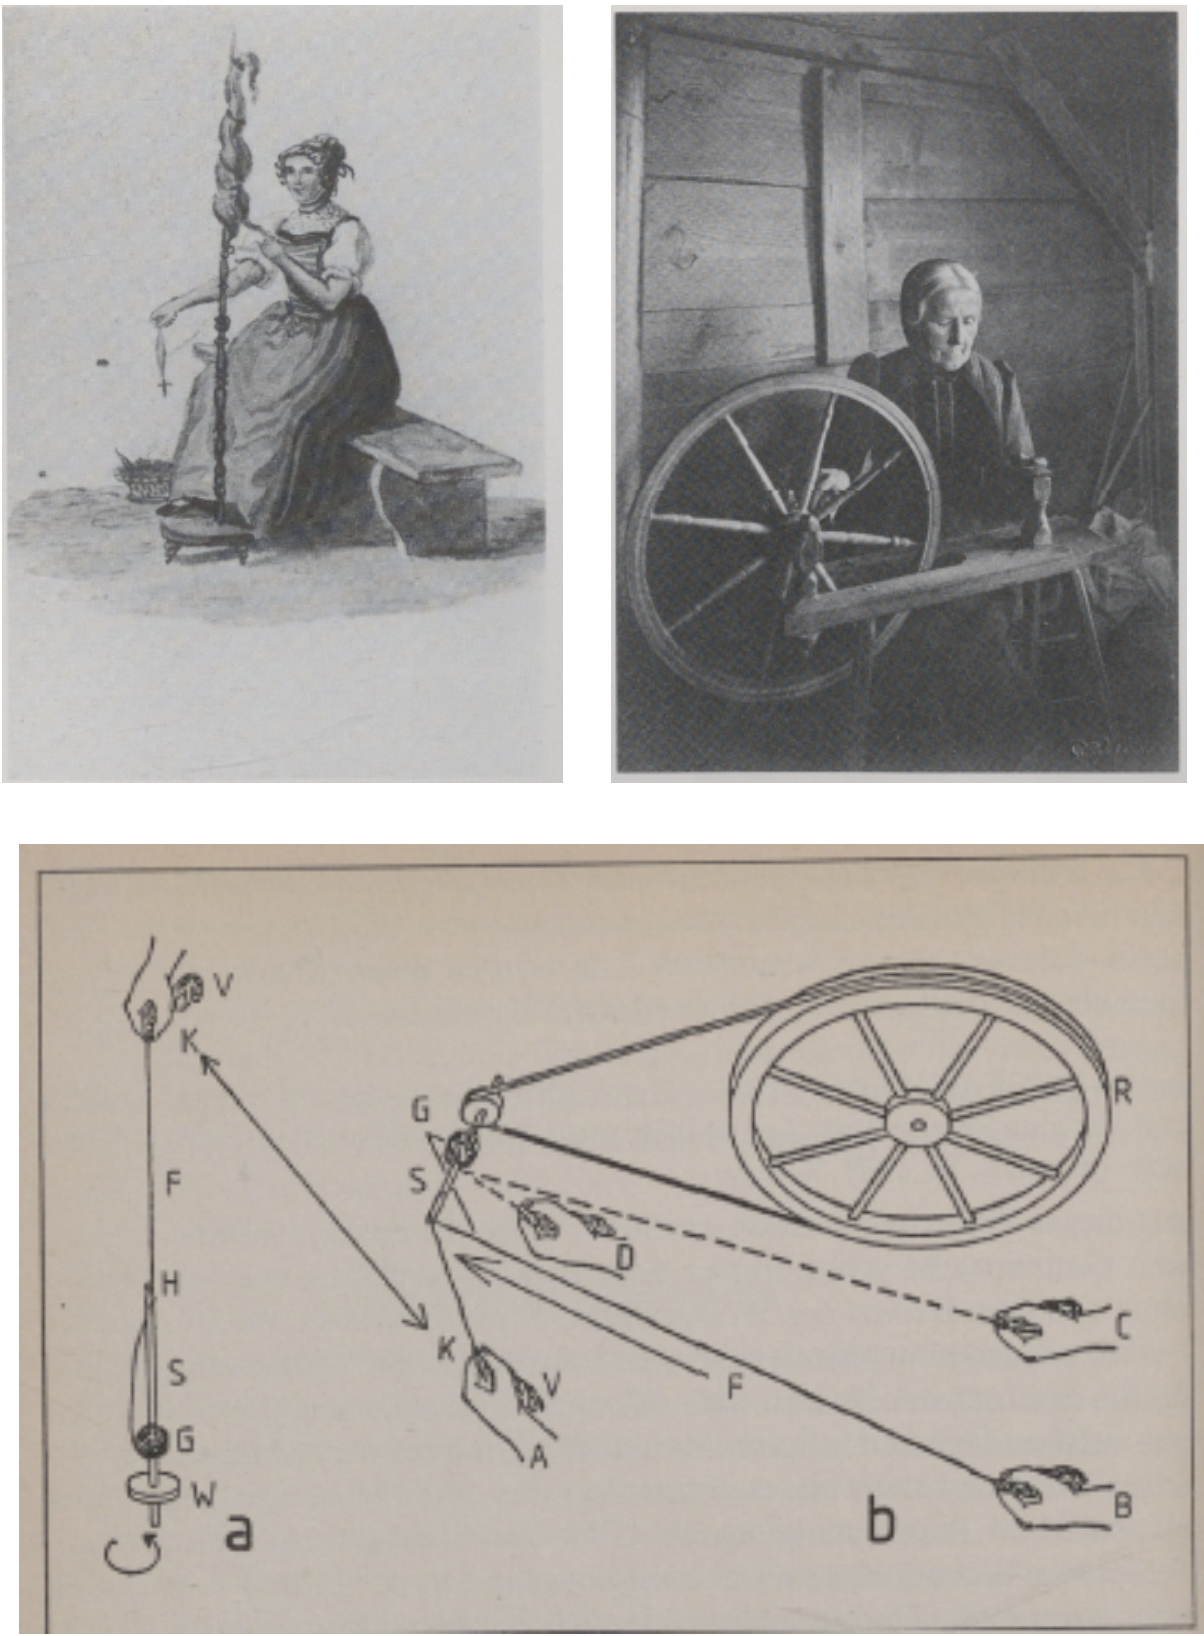
\includegraphics[width=0.7\linewidth]{images/spinning_jenny.png}
\end{center}
Ein zentrales Problem der vorindustriellen Textilproduktion war die Garnherstellung.

Das Spinnen war deutlich arbeitsintensiver als das Weben.

Dadurch entstand ein Produktionsengpass,
der zum Ausgangspunkt wichtiger technischer Innovationen wurde.

Entscheidend waren Entwicklungen aus Grossbritannien:

\begin{itemize}
    \item mechanische Spinnmaschinen wie die Spinning Jenny
    \item die Mule-Spinnmaschine
    \item später mechanische Webstühle
\end{itemize}

Diese Maschinen steigerten die Produktivität erheblich
und ermöglichten eine weitgehende Mechanisierung der Textilherstellung.

Der technische Fortschritt setzte somit zunächst nicht in der Schweiz,
sondern in Grossbritannien ein. 

\subsection{Warum begann die Industrialisierung in Grossbritannien?}

Grossbritannien gilt als Ursprungsland der Industrialisierung.

Von der Mitte des 18. bis zur Mitte des 19. Jahrhunderts
entstanden dort die grundlegenden industriellen Produktionsformen.

Die Mechanisierung breitete sich rasch aus:

\begin{itemize}
    \item Textilindustrie
    \item Maschinenbau
    \item Eisen- und Stahlproduktion
    \item Bergbau
    \item Chemieindustrie
    \item Energieversorgung
    \item Transportwesen
\end{itemize}

Gleichzeitig veränderte sich die Arbeitswelt grundlegend.

Maschinen konnten zunehmend von weniger qualifizierten Arbeitskräften bedient werden,
wodurch Frauen und Kinder verstärkt in die industrielle Produktion eingebunden wurden.

Die Industrialisierung führte ausserdem zu:

\begin{itemize}
    \item Konzentration von Kapital
    \item Entstehung moderner Unternehmen
    \item Ausbau der Kreditwirtschaft
    \item Zentralisierung der Produktion in Fabriken
    \item starkem Städtewachstum
\end{itemize}

Die industrielle Revolution war somit nicht nur eine technische,
sondern auch eine wirtschaftliche und gesellschaftliche Revolution. 

\subsection{Nachholende Industrialisierung in der Schweiz}

Die Schweiz übernahm viele Entwicklungen aus Grossbritannien.

Dieser Prozess wird als nachholende Industrialisierung bezeichnet.

Technologien und Organisationsformen wurden importiert
und an die lokalen Bedingungen angepasst.

Im Verlauf des 19. Jahrhunderts entstanden in der Ostschweiz:

\begin{itemize}
    \item Spinnereien
    \item Webereien
    \item Stickereifabriken
    \item Bleichereien
    \item Veredelungsbetriebe
\end{itemize}

Besonders wichtig war die Einführung des Fabriksystems.

Der Einsatz von Dampfkraft machte Produktionsstandorte
zunehmend unabhängig von Flüssen und Wasserkraft.

Dadurch beschleunigten sich Industrialisierung und Verstädterung erheblich. 

\begin{center}
    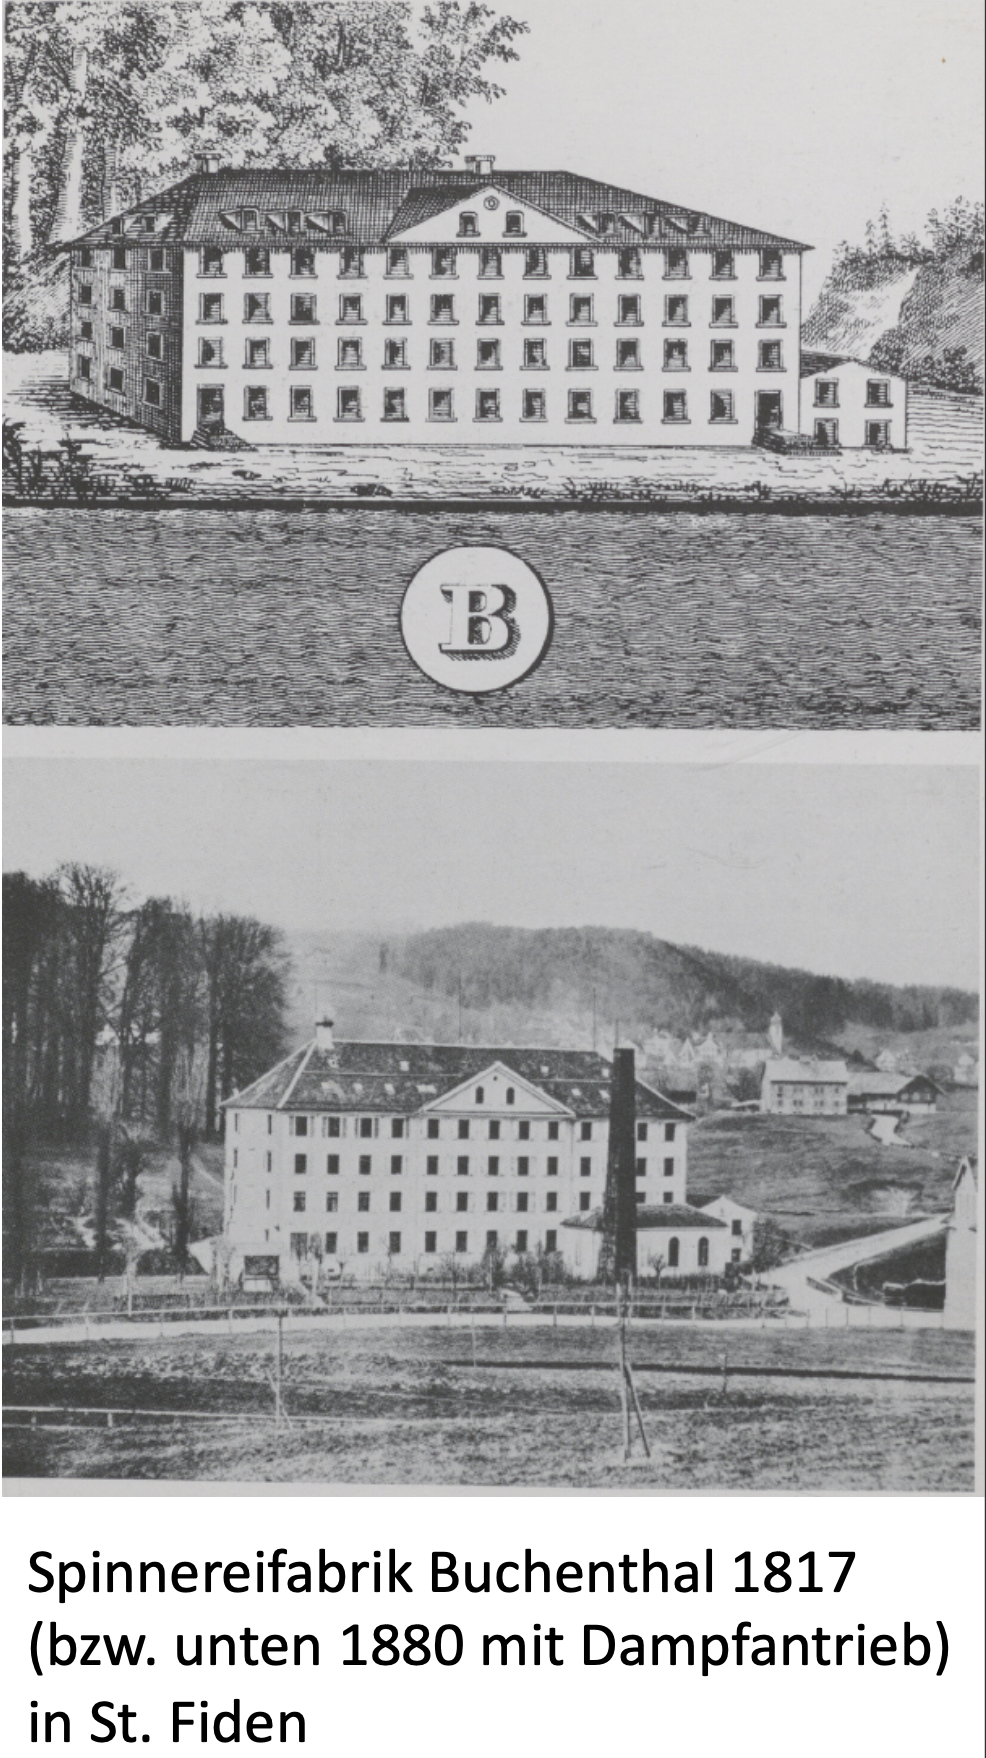
\includegraphics[width=0.8\linewidth]{images/spinnerei_buchental.png}
\end{center}

\subsection{Das Fabriksystem und die soziale Frage}

Mit der Industrialisierung entstanden neue Formen der Arbeit.

Die Fabrik wurde zum zentralen Ort der Produktion.

Damit verbunden waren zahlreiche soziale Probleme:

\begin{itemize}
    \item lange Arbeitszeiten
    \item Kinderarbeit
    \item geringe Arbeitssicherheit
    \item Disziplinierung durch Strafen und Entlassungen
    \item schlechte Arbeitsbedingungen
\end{itemize}

Gleichzeitig entwickelte sich eine neue Arbeiterkultur.

\begin{center}
    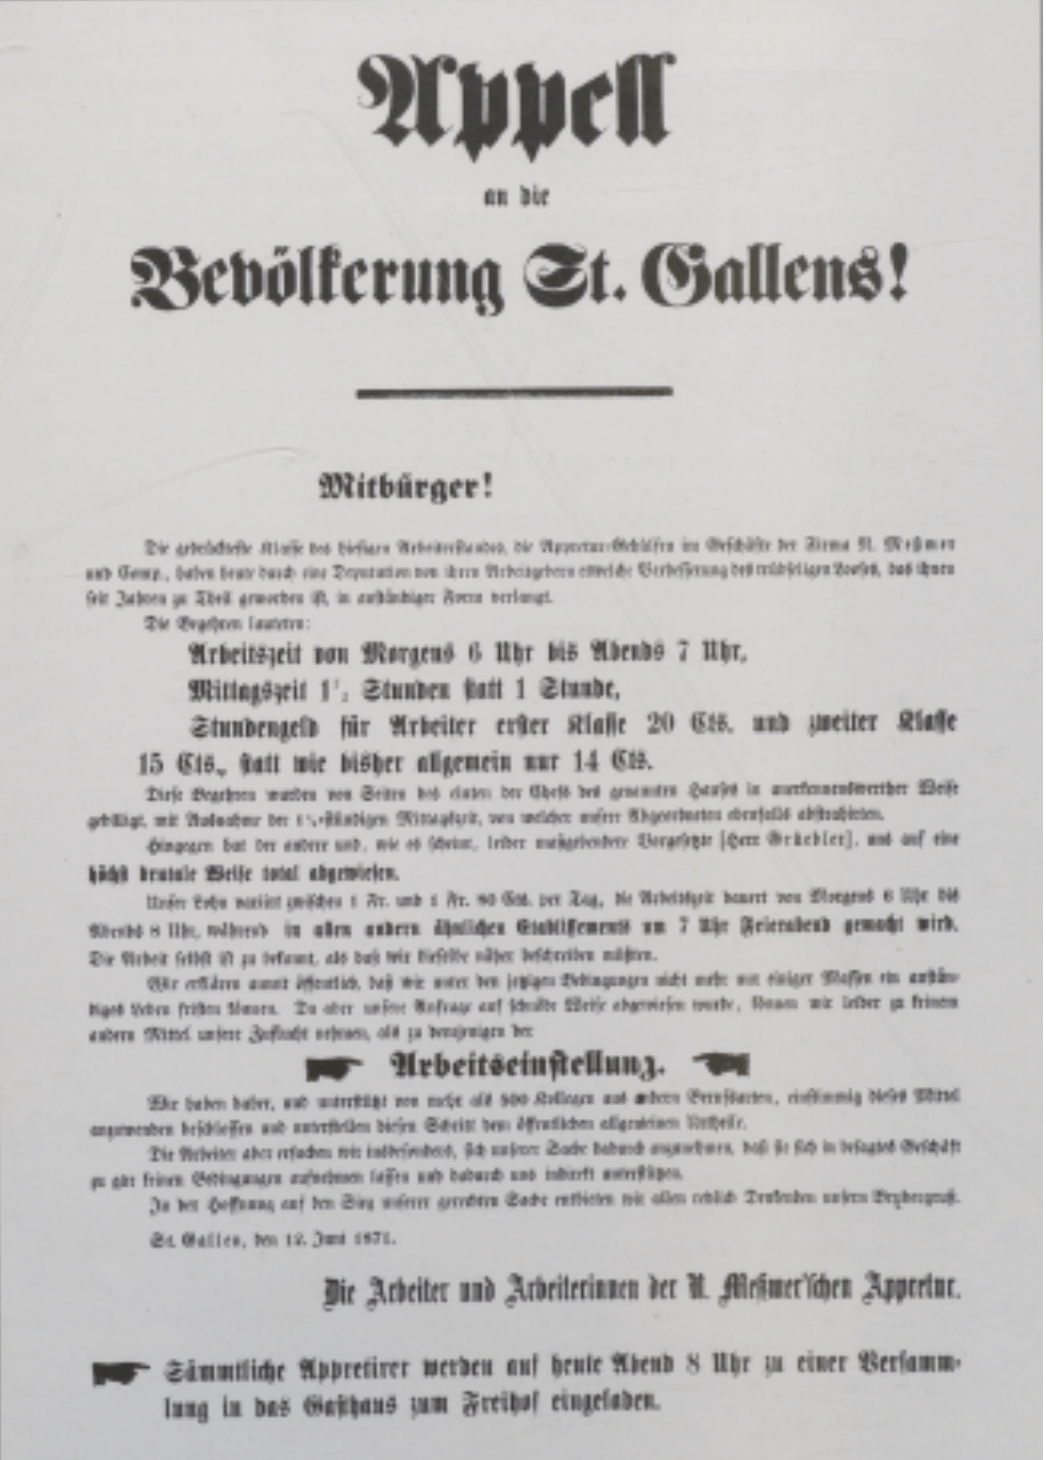
\includegraphics[width=0.6\linewidth]{images/streik_st_gallen_1971.png}
\end{center}

Arbeiterinnen und Arbeiter organisierten sich zunehmend,
bildeten Solidaritätsnetzwerke und führten Streiks durch.

Die Industrialisierung brachte daher sowohl wirtschaftlichen Fortschritt
als auch neue gesellschaftliche Konflikte hervor. 

\subsection{Das Fabrikgesetz von 1877}

Die sozialen Probleme führten schliesslich zu staatlichen Eingriffen.

Mit dem eidgenössischen Fabrikgesetz von 1877
wurden erstmals verbindliche Regeln für Fabriken geschaffen.

Wichtige Bestimmungen waren:

\begin{itemize}
    \item Verbot der Kinderarbeit
    \item Schutz von Gesundheit und Leben der Beschäftigten
    \item Einführung des Elfstundentages
    \item Unfallmeldepflicht
    \item Registrierung der Arbeitnehmer
    \item Regulierung von Disziplinarmassnahmen
    \item Kündigungsschutz
    \item Einführung staatlicher Fabrikinspektoren
\end{itemize}

Das Gesetz markiert einen wichtigen Schritt
vom weitgehend unregulierten Fabrikbetrieb
hin zu staatlich kontrollierten Arbeitsverhältnissen. 

\subsection{Die ostschweizerische Stickereiindustrie}

Im 19. Jahrhundert entwickelte sich die Stickerei
zum bedeutendsten Industriezweig der Ostschweiz.

Gründe dafür waren:

\begin{itemize}
    \item wachsender internationaler Wettbewerb
    \item Spezialisierung auf hochwertige Produkte
    \item hohe Nachfrage nach Stickereiwaren
\end{itemize}

Um 1910 exportierte die Schweiz Stickereien
im Wert von rund 200 Millionen Franken.

Mehr als 60'000 Menschen arbeiteten in den Regionen
St. Gallen, Appenzell und Thurgau in diesem Wirtschaftszweig. 

\subsection{Mechanisierung der Stickerei}

Auch die Stickerei wurde mechanisiert.

Die Einführung von Stickmaschinen ab etwa 1850
steigerte die Produktivität erheblich.

Eine einzelne Maschine konnte die Arbeit
zahlreicher Handstickerinnen ersetzen.

Mit der Schifflistickmaschine ab 1863
wurden zudem körperliche Belastungen reduziert.

Gleichzeitig brachte die Mechanisierung neue Formen der Arbeitsorganisation:

\begin{itemize}
    \item Arbeit nach Maschinentakt
    \item stärkere Arbeitsteilung
    \item höhere Produktionsleistung
\end{itemize}

Anders als in vielen anderen Industrien
blieb jedoch ein grosser Teil der Produktion
weiterhin in Heimarbeit organisiert. 

\begin{center}
    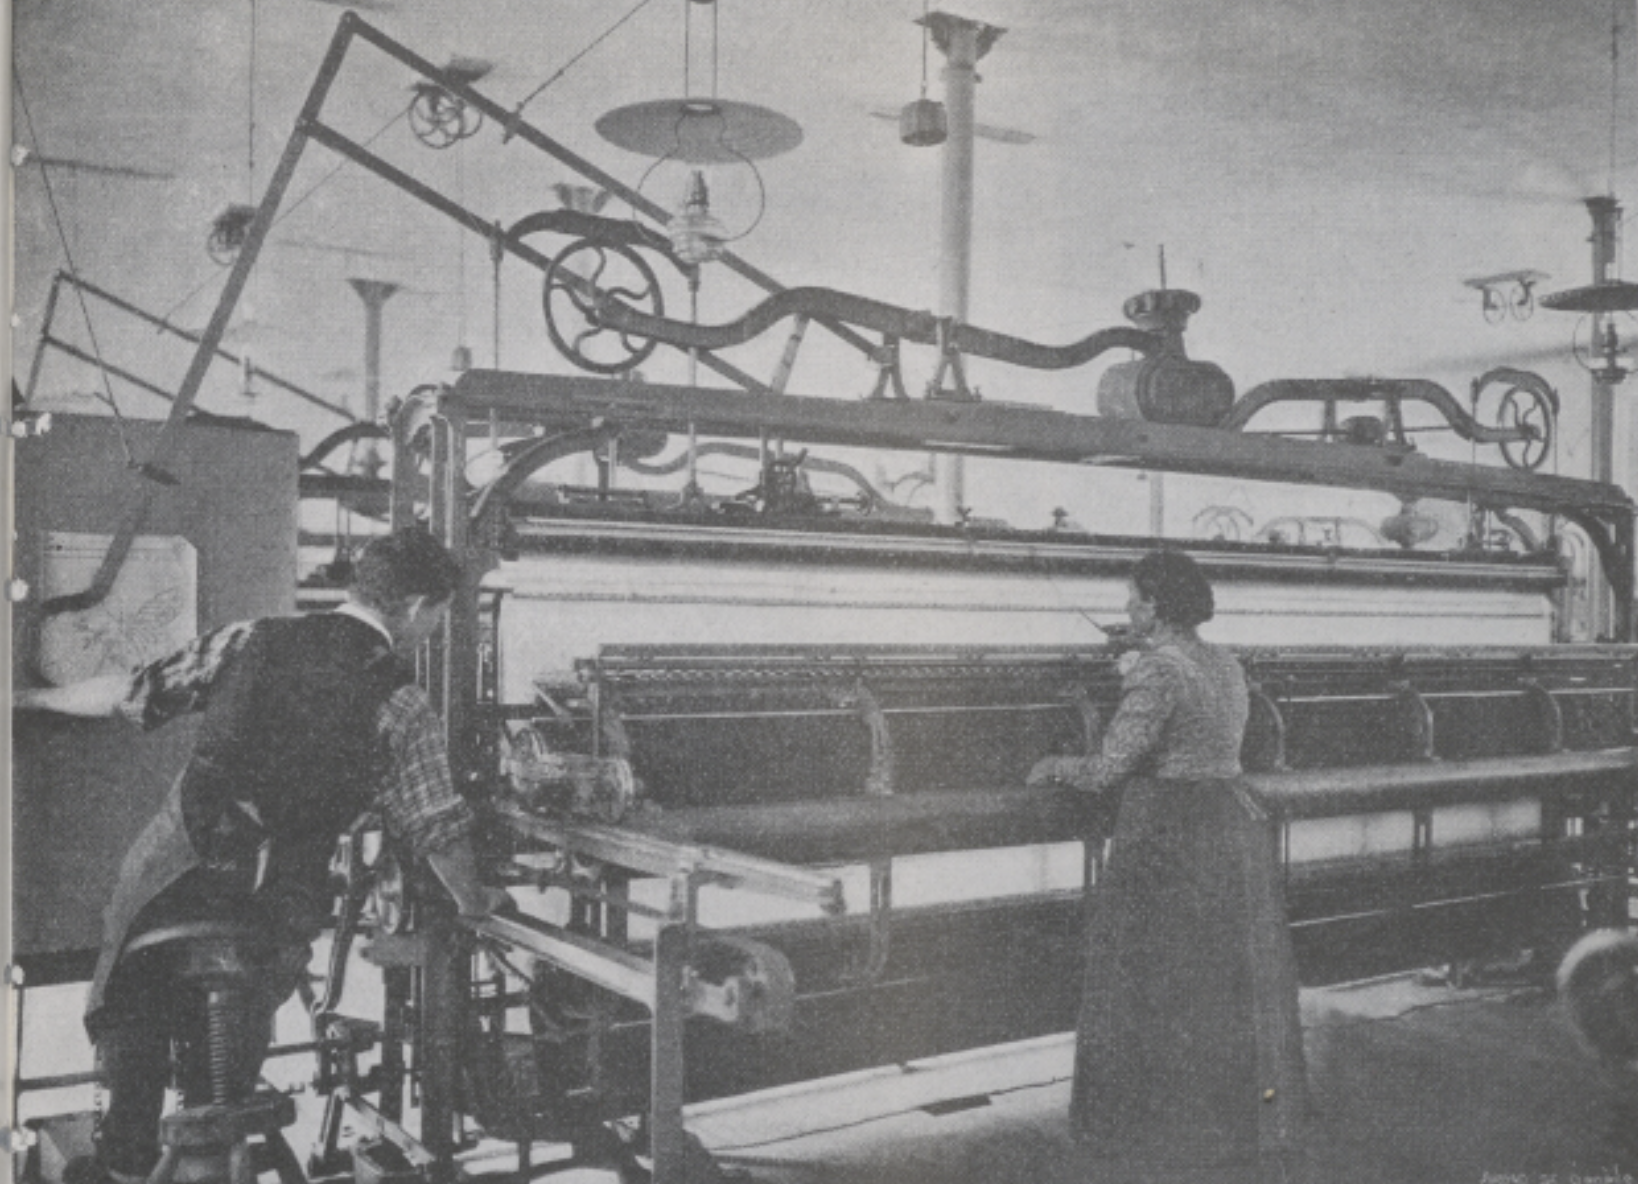
\includegraphics[width=0.8\linewidth]{images/schifflistickmaschine.png}
\end{center}

\subsection{Heimarbeit und das Dilemma der Moderne}

Viele Sticker entschieden sich bewusst gegen die Fabrikarbeit.

Die Heimarbeit versprach:

\begin{itemize}
    \item grössere Selbstständigkeit
    \item flexible Arbeitszeiten
    \item Arbeit im familiären Umfeld
\end{itemize}

Gleichzeitig entstanden neue Abhängigkeiten.

Heimarbeiter mussten:

\begin{itemize}
    \item Maschinen selbst finanzieren
    \item wirtschaftliche Risiken tragen
    \item sich den Vorgaben der Verleger unterordnen
    \item mit starken Marktschwankungen leben
\end{itemize}

Die Industrialisierung führte daher nicht zu einer einfachen Verbesserung der Lebensbedingungen.

Vielmehr entstand ein Spannungsverhältnis zwischen
Fabrikarbeit und scheinbar selbstständiger Heimarbeit.

Dieses Spannungsfeld bezeichnet die Vorlesung als das „Dilemma der Moderne“. 

\begin{center}
    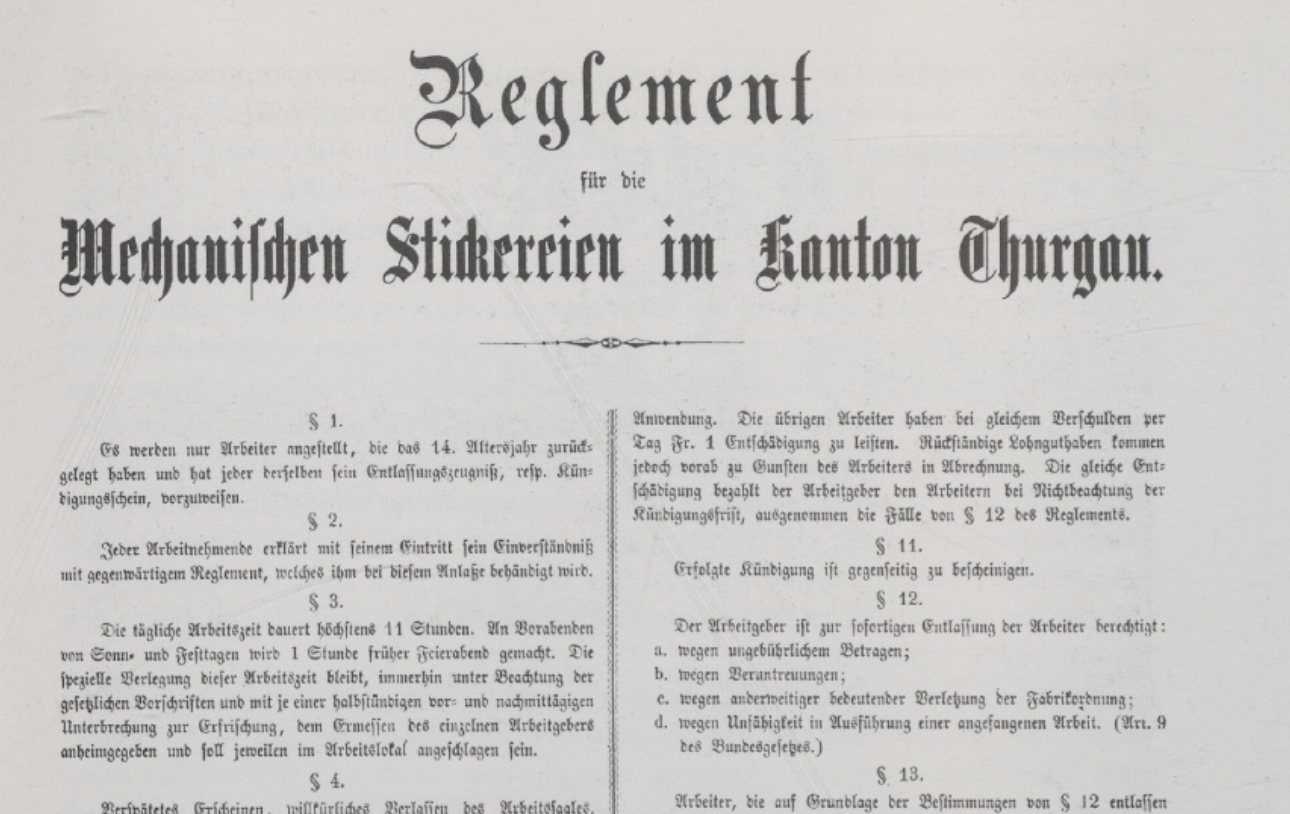
\includegraphics[width=0.6\linewidth]{images/fabrikreglement_stickerei.png}
\end{center}

\subsection{Arbeitsteilung und Geschlechterrollen}

Die Industrialisierung veränderte auch die Geschlechterordnung.

Frauen übernahmen zahlreiche Tätigkeiten
in Textil- und Stickereibetrieben.

Gleichzeitig blieb die Arbeit stark geschlechtsspezifisch organisiert.

Bestimmte Aufgaben wurden Männern,
andere Frauen zugewiesen.

Die industrielle Arbeitsteilung beeinflusste somit nicht nur die Produktion,
sondern auch gesellschaftliche Vorstellungen von Geschlecht und Arbeit. 

\subsection{Das Ende der Stickereiblüte}

Die ostschweizerische Stickerei war stark von Modetrends abhängig.

Nach dem Ersten Weltkrieg veränderten sich Geschmack
und Bekleidungsstile grundlegend.

Die sogenannte Neue Sachlichkeit der 1920er Jahre
bevorzugte schlichte und funktionale Kleidung.

Dadurch sank die Nachfrage nach aufwendigen Stickereien deutlich.

Die einstige Leitindustrie der Ostschweiz verlor ihre wirtschaftliche Bedeutung. 

\subsection{Zentrale Erkenntnisse}

Die Industrialisierung war weit mehr als die Einführung neuer Maschinen.

Sie führte zu tiefgreifenden Veränderungen in Wirtschaft,
Gesellschaft und Alltag.

Die Vorlesung zeigt insbesondere:

\begin{itemize}
    \item den Übergang von der Protoindustrie zum Fabriksystem
    \item die Bedeutung technischer Innovationen für Produktivitätssteigerungen
    \item die Entstehung neuer Arbeitsformen und sozialer Konflikte
    \item die Rolle staatlicher Regulierung
    \item die Wechselwirkungen zwischen Technik, Wirtschaft und Gesellschaft
\end{itemize}

Die zentrale These lautet:

Industrialisierung ist kein rein technischer Prozess.
Sie beschreibt einen umfassenden gesellschaftlichen Wandel,
in dem neue Technologien, wirtschaftliche Interessen und soziale Strukturen
aufeinander einwirken und die moderne Gesellschaft hervorbringen.